\documentclass[]{article}

\usepackage[italian]{babel}
\usepackage[margin=20mm, footskip = 20pt]{geometry}
\usepackage{array}
\usepackage{tabularx}
\usepackage{graphicx}
\usepackage{subfiles}
\usepackage{hyperref}
\usepackage{nameref}
\usepackage{titlesec}
\usepackage{longtable}
\usepackage[table]{xcolor}
\usepackage{titling}
\usepackage{lastpage}
\usepackage{ifthen}
\usepackage{calc}
\usepackage{soulutf8}
\usepackage{contour}
\usepackage{float}
\usepackage{fancyhdr}
\usepackage{multirow}
\usepackage{pgfgantt}
\usepackage{lscape}

\newcommand{\hr}{\par\vspace{-.1\ht\strutbox}\noindent\hrulefill\par}

\graphicspath{ {./}
	{./commons/res}
}

%--------------------------------------------------
% Comandi per inserire contenuto del documento
%--------------------------------------------------
\makeatletter

\newcommand\appendToGraphicsPath[1]{%
	\g@addto@macro\Ginput@path{{#1}}%
}

\newcommand{\setTitle}[1]{%
	\newcommand{\@phTitle}{#1}%
}
\newcommand{\phTitle}{\@phTitle}

\newcommand{\setDate}[1]{%
	\newcommand{\@phDate}{#1}%
}
\newcommand{\phDate}{\@phDate}

\newcommand{\setUso}[1]{%
	\newcommand{\@uso}{#1}%
}
\newcommand{\uso}{\@uso}

\newcommand{\setVersione}[1]{%
	\newcommand{\@versione}{#1}%
}
\newcommand{\versione}{\@versione}

\newcommand{\disabilitaVersione}{%
	\renewcommand{\setVersione}[1]{}%
	\renewcommand{\versione}{DISABILITATA}
}

\newcommand{\setResponsabile}[1]{%
	\newcommand{\@responsabile}{#1}%
}
\newcommand{\responsabile}{\@responsabile}

\newcommand{\setRedattori}[1]{%
	\newcommand{\@redattori}{#1}%
}
\newcommand{\redattori}{\@redattori}

\newcommand{\setVerificatori}[1]{%
	\newcommand{\@verificatori}{#1}%
}
\newcommand{\verificatori}{\@verificatori}

\newcommand{\setModifiche}[1]{%
	\newcommand{\@modifiche}{#1}%
}
\newcommand{\modifiche}{\@modifiche}

\makeatother 

%--------------------------------------------------
% Comandi per i documenti esterni e il glossario
%--------------------------------------------------

\newcommand{\dext}[1]{\textsc{#1\textsubscript{\textit{D}}}}

\newcommand{\glock}[1]{\textsc{#1\textsubscript{\textit{G}}}}

%--------------------------------------------------
% Comandi per impostare sottotitoli di quarto e quinto livello
%--------------------------------------------------

\setcounter{secnumdepth}{4}
\setcounter{tocdepth}{4}

\titleformat{\paragraph}
{\normalfont\normalsize\bfseries}{\theparagraph}{1em}{}
\titlespacing*{\paragraph}{0pt}{2.25ex plus 1ex minus .2ex}{1.5ex plus .2ex}

\titleformat{\subparagraph}
{\normalfont\normalsize\bfseries}{\thesubparagraph}{1em}{}
\titlespacing*{\subparagraph}{0pt}{1.75ex plus 1ex minus .2ex}{.75ex plus .1ex}

\appendToGraphicsPath{../../../commons/res/}

%------------------------------
%
% COMANDI DI CONFIGURAZIONE
%
%------------------------------

\setTitle{Verbale riunione \#19}

\setVersione{1.0.0}

\setDate{03-01-2021}

\setResponsabile{Valton Tahiraj}

\setRedattori{Alessandro Dindinelli}

\setVerificatori{Giacomo Bulbarelli}

\setUso{Interno}

\setModifiche{
	1.0.0 & Valton Tahiraj & Responsabile & 9-01-2020 & Approvazione documento\\
	0.1.0 & Giacomo Bulbarelli & Verificatore & 04-01-2021 & Verifica documento\\
	0.0.0 & Alessandro Dindinelli & Redattore & 03-01-2021 & Stesura iniziale}

\begin{document}

	% Direttive per la creazione del titolo tramite comando maketitle
\title{\huge \textsc{\phTitle{}} \\
	\vspace{11pt} \large \textsc{\phDate{}}}

\author{} % Non toccare
\date{} % Non toccare

%--------------------
% Frontespizio
%--------------------

% Logo del gruppo
\begin{figure}[t!]
	\centering
	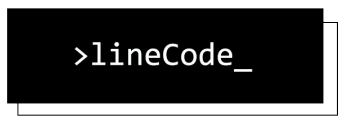
\includegraphics[width=20em]{lclong}
\end{figure}

% Titolo / Nome
\maketitle
\thispagestyle{empty}

% Dati specifici sul doc in forma tabulare
\begin{table}[ht]
	\begin{center}
		\label{tab:Dati sul documento}
		\begin{tabular}{r|l}
			\multicolumn{2}{c}{ \textsc{Dati sul documento} } \\
			\hline
			\textbf{Versione} & \versione{} \\
			\textbf{Uso} & \uso{}  \\
			\textbf{Redattori} & \redattori{} \\
			\textbf{Verificatori} & \verificatori{} \\
			\textbf{Responsabile} & \responsabile{} \\
			\textbf{Destinatari} & lineCode \\
								& prof.\ Vardanega Tullio \\		
								& prof.\ Cardin Riccardo \\
			\ifthenelse{\equal{\uso}{Esterno}}{
								& Sanmarco Informatica
			}{} \\
		\end{tabular}
	\end{center}
\end{table}

\newpage

\renewcommand{\arraystretch}{2} % allarga le righe con dello spazio sotto e sopra
\begin{longtable}[H]{>{\centering\bfseries}m{2cm} >{\centering}m{3.5cm} >{\centering}m{2.5cm} >{\centering}m{3cm} >{\centering\arraybackslash}m{5cm}}
	\rowcolor{lightgray}
	{\textbf{Versione}} & {\textbf{Nominativo}} & {\textbf{Ruolo}} & {\textbf{Data}} & {\textbf{Descrizione}}  \\
	\endfirsthead%
	\rowcolor{lightgray}
	{\textbf{Versione}} & {\textbf{Nominativo}}  & {\textbf{Ruolo}} & {\textbf{Data}} & {\textbf{Descrizione}}  \\
	\endhead%
	\modifiche{}%
\end{longtable}

	\newpage

	\section{Introduzione}
		\subsection{Luogo e data dell'incontro}
		\begin{itemize}
			\item \textbf{Modalità}: Telematica;
			\item \textbf{Software utilizzato}: \glock{Discord};
			\item \textbf{Data}: 03 Gennaio 2021;
			\item \textbf{Ora di inizio}: 10:00;
			\item \textbf{Ora di fine}: 12:00.
		\end{itemize}

		\subsection{Presenze}
		\begin{itemize}
			\item \textbf{Presenti}:
		\begin{itemize}
			\item Matteo Alba
			\item Giacomo Bulbarelli
			\item Alessandro Chimetto
			\item Alessandro Dindinelli
			\item Lucia Fenu
			\item Paolo Scanferlato
			\item Valton Tahiraj
		\end{itemize}
			\item \textbf{Assenti}:
			\begin{itemize}
				\item Nessuno
			\end{itemize}
		\end{itemize}

		\subsection{Ordine del giorno}
		\begin{enumerate}
            \item discussione sullo stato dei lavori per la redazione del documento \dext{Analisi dei Requisiti};
            \item discussione su dettagli implementativi del sistema per la redazione dei casi d'uso;
            \item suddivisione lavori per i prossimi documenti da produrre;
            \item varie ed eventuali.
		\end{enumerate}

	\newpage

	\section{Svolgimento}
		\subsection{Discussione sullo stato dei lavori}
        Ogni componente ha specificato il proprio stato di avanzamento per i compiti che gli erano stati assegnati, e si è passati poi ha decidere un ordine numerico assoluto da dare ai casi d'uso.\\

        \subsection{Discussione dettagli implementativi del sistema}
        Si è discusso sui principi di come implementare la coda degli ordini che sarà poi assegnata ad ogni unità robot, decidendo di permetterne una modifica solo in caso l'unità sia alla base. Per quanto riguarda la creazione e modifica della mappa si è deciso di implementarla tramite file testuale da importare nel sistema.\\
        
        \subsection{Suddivisione lavori prossimi documenti}
        Si è deciso di iniziare uno sviluppo parallelo per il documento \dext{Piano di Qualifica} che verrà portato avanti inizialmente dai membri del gruppo che non hanno attualmente compiti legati al redigere il documento \dext{Analisi dei Requisiti}. \\
        I componenti del gruppo che si stanno occupando dei casi d'uso avranno poi il compito di redigere anche i requisiti che ne derivano.\\

		\subsection{Fissata riunione successiva}
		Riunione successiva fissata in:
		\begin{itemize}
			\item \textbf{Data}: 05-01-2021;
			\item \textbf{Ora}: 10:00;
			\item \textbf{Modalità}: Telematica: \glock{Discord}.
		\end{itemize}

	\newpage

	\section{Tabella delle decisioni}

		\begin{table} [h!]
			\rowcolors{2}{gray!25}{gray!6}
			\begin{center}
				\begin{tabular} { m{2cm} m{14cm} }
					\rowcolor{lightgray}
					\textbf{ID} & \textbf{Decisione}\\
					V19.1 & Si è scelta una numerazione progressiva per i casi d'uso, partendo da quelli che non richiedono autenticazione al sistema, aumentando poi al crescere dei privilegi utente richieste, terminando quindi con quelli legati all'amministrazione di sistema.\\
					V19.2 & Le unità robot saranno implementate con una lista di ordini da soddisfare, che potrà essere modificata solo quando queste si troveranno alla base.\\
					V19.3 & La realizzazione e modifica della mappatura dell'ambiente verrà realizzata tramite importazione di un file testuale formattato appositamente.\\
					V19.4 & Per la redazione parallela di altri documenti i compiti sono stati suddivisi nel seguente modo:
					\begin{itemize}
						\item l'impostazione iniziale del \dext{Glossario} è stata affidata a Paolo Scanferlato;
						\item la redazione della prima parte del \dext{Piano di Qualifica} è stata divisa tra Matteo Alba e Lucia Fenu.
					\end{itemize}\\
				\end{tabular}
			\end{center}
		\end{table}

\end{document}

